\documentclass[number]{notes}
\usepackage{titlepage}
\usepackage{ncolor}
\usepackage{math}
\usepackage{enumitem}
\usepackage{multicol}
\usepackage{float}
\usepackage{pdflscape}
\usepackage{listings}

\lstdefinestyle{customc}{
  belowcaptionskip=1\baselineskip,
  breaklines=true,
  frame=l,
  xleftmargin=\parindent,
  language=C,
  showstringspaces=false,
  basicstyle=\footnotesize\ttfamily,
  keywordstyle=\bfseries\color{green!40!black},
  commentstyle=\itshape\color{purple!40!black},
  identifierstyle=\color{blue},
  stringstyle=\color{orange},
  numbers=left
}
\lstset{escapechar=@,style=customc}

\setprimary{purple}

\name{Daniel}{Fitzmaurice}
\studentnumber{43961229}
\coursecode{csse2310}

\linespread{1}
\setlength{\columnseprule}{0.4pt}

\begin{document}
\begin{landscape}
\headfoot
\begin{multicols}{3}

\heading{Function Pointers}
\texttt{int (*fp)(int, char*)} - Declares fp to be a pointer to a function which takes int and char* arguments and returns int\\
\texttt{void (*fp2[10])(double)} - Declares fp2 to be an array (of size 10) of pointers to functions taking a double parameter and returning nothing\\
\texttt{int (*fp3)()} - Declares fp3 to be a pointer to a function returning int. Argument types unknown and won't be checked by the compiler (Up to programmer to use this correctly).

\heading{Storage classes}
\subheading{auto}
\begin{itemize}[nolistsep]
    \item Variable has local (automatic) extent, i.e. removed at end of block
    \item Permitted within a block only (i.e. not top level)
    \item This is the default so rarely seen
\end{itemize}
\subheading{extern}
\begin{itemize}[nolistsep]
    \item Variable/function is external to all functions, i.e. can be accessed by name by any function
    \item Globally accessible - linker must know about the name
    \item Must be defined once somewhere (can be declared anywhere)
\end{itemize}
\subheading{register}
\begin{itemize}[nolistsep]
    \item Hint to compiler to put variable in a register, otherwise like auto
\end{itemize}
\subheading{static}
\begin{itemize}[nolistsep]
    \item Name is only accessible in this file (i.e. not exported to linker)
    \item For variables - extent is static - variable lasts for life of program
\end{itemize}

\heading{5 Views of OS}
\begin{enumerate}[nolistsep]
    \item Hardware
    \item Operating System Designer
    \item Application Programmer
    \item End-User
    \item System Administrator
\end{enumerate}

\heading{Environment Variables}
\textbf{HOME} - full pathname of home directory\\
\textbf{PATH} - colon separated list of pathnames to search for commands\\
\textbf{USER} - your username\\
\textbf{SHELL} - full pathname of your login shell
\subheading{Local Variable}
\texttt{courseCode=CSSE2310}\\
\subheading{Environment Variable}
\texttt{export courseCode}

\heading{Metacharacters}
\subheading{WildCards}
\textbf{*} - zero or more characters\\
\textbf{?} - any single character\\
\subheading{Comment}
\textbf{\#} - start of comment (goes till end of line)
\subheading{Running Commands}
\textbf{\&} - run command in background\\
\textbf{;} - used to separate commands\\
\textbf{`command`} - substitute result of running command
\subheading{Variable Substitution}
\textbf{\$varname} - substitute value of variable
\subheading{SubShell}
\textbf{(...commands...)} - execute commands in a sub-shell
\subheading{Conditional sequences}
\textbf{||} - execute command if previous command failed\\
\textbf{\&\&} - execute command if previous one succeeded\\
A success is when the program returns an exit code 0
\subheading{Redirection and Pipes}
\textbf{|} - pipe, output of one program sent to the input of the next\\
\textbf{>} - send stdout to file\\
\textbf{<} - write stdin from file\\
\textbf{>>} - append stdout to file
\subheading{Quoting}
Single Quotes - inhibit wildcard replacement, variable substitution, command substitution.\\
Double Quotes - inhibit wildcard replacement only.\\
Can also use backslashes.

\heading{Shell Scripting}
\subheading{Shell Arithmetic}
Use \texttt{expr EXPRESSION} command. Result is printed to stdout.
\subheading{Shell Conditional}
Use \texttt{text EXPRESSION} or \texttt{[ EXPRESSION ]}. \texttt{EXPRESSION} follows \texttt{INT1 option INT2} where option can be: \texttt{-eq} (equals), \texttt{-ge} (greater than or equal), \texttt{-gt} (greater than), \texttt{-le} (less than or equal), \texttt{-lt} (less than), \texttt{-ne} (not equal). Result is exit code 1 for false and 0 for true.
\subheading{Control Structures}
\subsubheading{For Loop}
\texttt{for name [ in \textit{word...} ]\\do\\\textit{commands...}\\done}
If words omitted, uses script arguments.\\
\subsubheading{While Loop}
\texttt{while \textit{command1}\\do\\\textit{command2}\\done}\\
\subsubheading{If Then Else}
\texttt{if \textit{command1}\\then\\\textit{command2}\\elif \textit{command3}\\then\\\textit{command4}\\else\\\textit{command5}\\fi}\\
\subsubheading{Other Control Structures}
Case. Until - do - done. Done.


\heading{Built-in Shell Variables}
\textbf{\$\$} - process ID of shell\\
\textbf{\$0} - name of the shell script\\
\textbf{\$1\ldots\$9} - command line arguments\\
\textbf{\$*} - all the command line arguments\\
\textbf{\$\#} - number of command line arguments (excludes command name)\\
\textbf{\$?} - exit status of last command\\
\textbf{\$!} - process ID of last background command

\heading{Paging}
One of several methods of implementing virtual memory. Divide physical memory into fixed-sized blocks called page frames (size is power of 2, usually between 512 bytes and 8192 bytes). Divide logical memory into blocks of same size called pages. Keep track of all free frames. To run a program of n pages, need to find n free frames and load program. Set up a page table to translate logical to physical addresses.
\subheading{Address Translation Scheme}
\textbf{Page Number} (p) - used as an index into a page table which contains base address of each page in physical memory\\
\textbf{Page Offset} (d) - combined with base address to define the physical memory address that is sent to the memory unit
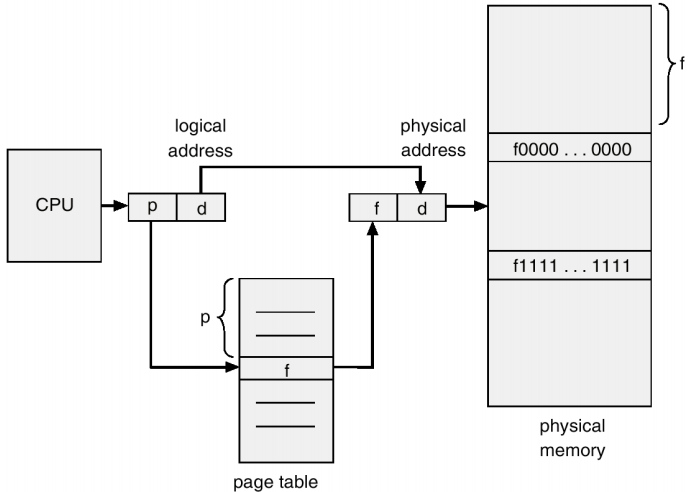
\includegraphics[width=0.5\linewidth]{pageTable.png}
\subheading{Implementation of Page Table}
Page table is kept in main memory. The two memory access problem can be solved by the use of a special fast-lookup hardware cache called associative memory or translation look-aside buffers (TLBs)
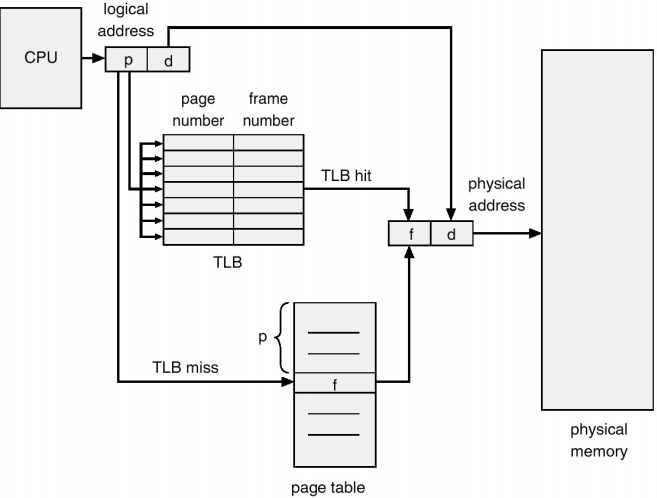
\includegraphics[width=\linewidth]{TLB.png}
\subsubheading{Page Faults}
If the TLB entry doesn't exist, then load it into the table
\subheading{Memory Protection}
Memory protection implemented by associating protection bit with each frame.
\subheading{Segmentation Faults}
Segmentation Fault arises when: Accessing invalid memory page, Trying to write to a read-only page.
\subheading{Shared Pages}
\subsubheading{Shared code}
One copy of read-only code shared among processes. Shared code must appear in same location in the virtual address space of all processes.\\
\subsubheading{Private code and data}
Each process keeps a separate copy of the code and data. The pages for the private code and data can appear anywhere in the virtual address space.
% TODO: add page table calc examples
\subheading{User-space vs Kernel}
The operating system controls the address ranges (pages) a process can use. It does not decide how that space is used. Management of those pages is the responsibility of the process (Usually vie standard libraries).

\heading{Memory-Related Bugs}
\begin{itemize}
    \item Dereferencing bad pointers
    \item Reading uninitialized memory
    \item Overwriting memory
    \item Referencing nonexistent variables
    \item Freeing blocks multiple times
    \item Referencing freed blocks
    \item Failing to free blocks
\end{itemize}

\heading{Processes}
\subheading{fork}
\texttt{int fork(void)} - creates a new process. Returns 0 to the child process else return child's pid.\\
Common for the parent to be the only one to continue forking
\subheading{exit}
\texttt{void exit(int status)} - exits a process (status 0 for no error)\\
\texttt{\_exit()} - will not run the registered exit functions
\subheading{atexit}
\texttt{atexit(void (*func)(void))} - registers functions to be executed upon exit. Functions called in reverse order of registration.
\subheading{wait}
\texttt{int wait(int\* child\_status)} - suspends process until child process terminates. Return the exit code, if child\_status is \texttt{NULL} then any child process.
\subheading{waitpid}
\texttt{waitpid(pid, \&status, options)} - can wait for a specific process. Various options (default is 0)
\subheading{exec}
\texttt{int execl(char *path, char *arg0, char *arg1, ..., 0)} - loads and runs executable at path with args arg0, arg1... (path is the complete path of the executable, arg0 becomes the name of the process).
\subsubheading{exec variations}
\texttt{execl()}, \texttt{execve()}, \texttt{execv()}, \texttt{execlp()}, \texttt{execle()}, \texttt{execvp()}\\
\textbf{l} - arguments directly in call (list)\\
\textbf{v} - arguments in array (vector)\\
\textbf{p} - use PATH to find program\\
\textbf{e} - provide environment definition
\subheading{Resource Sharing}
\begin{itemize}
    \item Parent and children share all resources
    \item Children share subset of parent's resources
    \item Parent and child share no resources
\end{itemize}
\subheading{Unix Process Hierarchy}
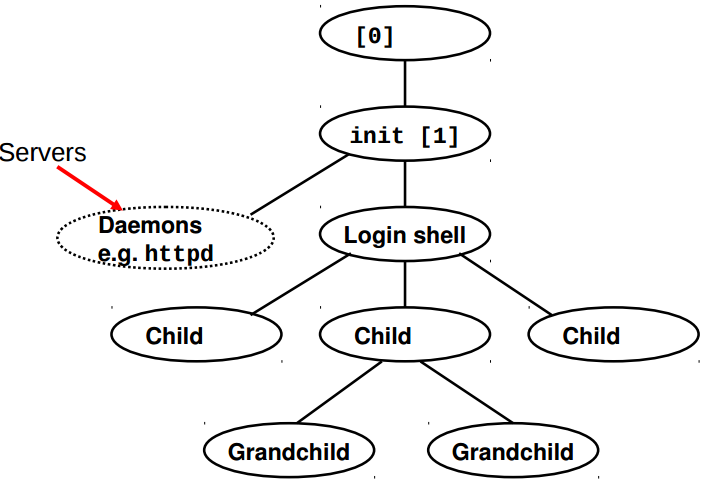
\includegraphics[width=\linewidth]{processHierarchy.png}

\heading{Files}
\subheading{Unix File Types}
\subsubheading{Regular file}
Binary or text file. Unix does not know the difference
\subsubheading{Directory file}
A file that contains the names and locations of other files
\subsubheading{Links}
Symbolic links to other files
\subsubheading{Character special and block special files}
Terminals (character special) and disks (block special)
\subsubheading{FIFO (named pipe)}
A file type used for interprocess communication
\subsubheading{Socket}
A file type used for network communication between processes
\subheading{Sharing Files}
A child process inherits its parent's open files. \texttt{refcnt} counts the number of references.

\heading{Piping}
\subheading{I/O Redirection}
\subsubheading{dup2}
\texttt{dup2(oldfd, newfd)} - copies per-process descriptor table entry oldfd to entry newfd.
\subheading{Example}
\begin{minipage}{\linewidth}
\begin{lstlisting}
int fdInput[2], fdOutput[2];
if (pipe(fdInput) == 0 && pipe(fdOutput) == 0) {
    int pid = fork();
    if (pid == 0) {
        //Child
        close(fdOutput[1]);
        close(fdInput[0]);
        dup2(fdOutput[0], STDIN_FILENO);
        dup2(fdInput[1], STDOUT_FILENO);
        if (execl(processName, processName, arg1,
                arg2, NULL) == -1) {
            error(SUBPROCESS_ERROR);
        }
    } else {
        //Parent
        childPid = pid;
        close(fdInput[1]);
        close(fdOutput[0]);
        input = fdopen(fdInput[0], "r");
        output = fdopen(fdOutput[1], "w");
    }
}
return
\end{lstlisting}
\end{minipage}

\heading{Threads}
A process may have multiple threads of control. Threads share code, data, open files etc (they have separate control flows).
\subheading{Threads vs Processes}
\subsubheading{Similarities}
Each has its own logical control flow. Each can run concurrently. Each is context switched.
\subsubheading{Differences}
Threads share code and data, processes (typically) do not. Threads are somewhat less expensive than processes.
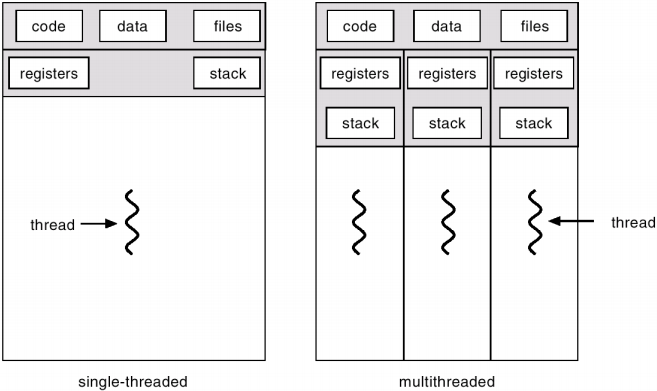
\includegraphics[width=\linewidth]{singlevsmulti.png}
\subheading{Multithreading Models}
\subsubheading{Many-to-One (User Threads)}
Threads implemented in user space. OS knows nothing about them\\
\subsubheading{One-to-One}
Threads implemented in kernel space, one kernel thread per user thread\\
\subsubheading{Many-to-Many}
Hybrid model
\subheading{Functions}
\subsubheading{pthread\_create}
\texttt{pthread\_create} takes a function pointer to start the thread\\
\subsubheading{pthread\_join}
\texttt{pthread\_join} waits for a specific thread
\begin{lstlisting}
int main() {
    pthread_t tid;
    pthread_create(&tid, NULL, thread1, NULL);
    pthread_join(tid, NULL);
    printf("Hello from first\n");
    exit(0);
}

void* thread1(void* vargp) {
    printf("Hello from second\n");
    return NULL;
}
\end{lstlisting}
\subsubheading{pthread\_self}
Returns the ID of the calling thread\\
\subsubheading{pthread\_exit}
Exits the calling thread\\
\subsubheading{pthread\_cancel}
\texttt{int pthread\_cancel(pthread\_t thread)} - sends a cancel request to thread\\
\subsubheading{pthread\_detach}
\texttt{int pthread\_detach(pthread\_t thread)} - marks the thread as detached\\
\subsubheading{pthread\_join}
\texttt{int pthread\_join(pthread\_t thread, void ** retval)} - waits for thread to finish
\subheading{Thread Lifecycle}
Ready $\rightarrow$ Running $\rightarrow$ Blocked $\rightarrow$ Terminated

\heading{Shared Data}
\textbf{Global variables} - one copy per process\\
\textbf{Local variables} - one copy per thread\\
\textbf{Static variables} - one copy per process
\subheading{Critical Section}
A critical section of a thread is a segment of code that shouldn't be interleaved with another thread's critical section. \textit{Note that these threads could be in different processes.} Concurrent access to shared data may result in data inconsistency.
\subsubheading{Semaphores}
Associate a semaphore S initially 1, with each shared variable (or set of shared variables). Surround corresponding critical section with \texttt{wait(S)} and \texttt{signal(S)} operations. This is a binary semaphore. Semaphore ensures mutually exclusive access to critical region.

\heading{Networking}
\subheading{Client-Server Model}
Most network applications are based on the client-server model: A server process and one or more client processes.
\subheading{TCP/IP}
Protocol = Rules for communication\\
TCP = Transmission Control Protocol. Provides communication between ports on two computers (bidirectional, point-to-point, reliable, byte stream). Uses IP (Internet Protocol) to transmit small packets of data between two IP addresses.
\subsubheading{TCP Connections}
Identified by: Source IP address, Source port number, Destination IP address, Destination port number.\\
\subsubheading{IP Addresses (v4)}
32-bit numbers. Often written in dotted decimal notation for human consumption (e.g. 130.102.2.15)
\subsubheading{Port Numbers}
16 bits: 0 - 65535. Below 1024, well known ports, reserved for standard services.
\subsubheading{Sockets}
A socket is a communication endpoint; associated with a file descriptor in UNIX - can do file I/O on socket, main distinction between regular file I/O and socket I/O is how the application ``opens'' the socket descriptors.
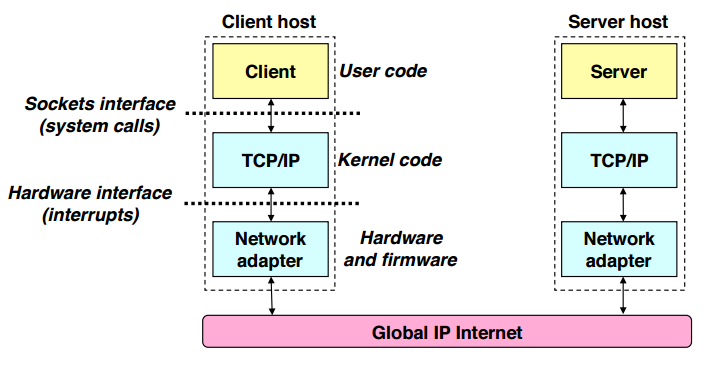
\includegraphics[width=\linewidth]{sockets.png}
\texttt{socket(...)} - create a new communication end-point\\
\texttt{bind(...)} - attach a local address to a socket\\
\texttt{listen(...)} - willing to accept connections, give queue size\\
\texttt{accept(...)} - wait for a connection attempt to arrive\\
\texttt{connect(...)} - attempt to establish a connection\\
\texttt{send(...)} or \texttt{write(...)} - send data over the connection\\
\texttt{recv(...)} or \texttt{read(...)} - receive data over the connection\\
\texttt{sendto(...)} - send datagram (UDP)\\
\texttt{recvfrom(...)} - receive datagram (UDP)\\
\texttt{close(...)} - release the connection\\
\texttt{shutdown(...)} - close down one side of connection (or both sides)
\subsubheading{Creating a Socket}
\texttt{AF\_INET} - indicates that the socket is associated with Internet Protocols\\
\texttt{SOCK\_STREAM} - selects a reliable byte stream connection (TCP)
\begin{lstlisting}
int fd = socket(AF_INET, SOCK_STREAM, 0);
if (fd < 0) {
    perror("Socket creation failed");
    exit(1);
}
\end{lstlisting}
\subsubheading{Socket Address Structures}
Generic socket address:
\begin{lstlisting}
struct sockaddr {
    sa_family_t sa_family; /* protocol family */
    char sa_data[14]; /* address data */
};
\end{lstlisting}
Internet-specific socket address:
\begin{lstlisting}
struct sockaddr_in {
    sa_family_t sin_family;
    /* address family (always AF_INET) */
    in_port_t sin_port;
    /* port num in network byte order */
    struct in_addr sin_addr;
    /* IP addr in network byte order */
    unsigned char sin_zero[8];
    /* pad to sizeof(struct sockaddr) */
};
\end{lstlisting}
\subsubheading{Accepting a request}
Blocks waiting for a connection request
\begin{lstlisting}
int listenfd; /* listening descriptor */
int connfd; /* connected descriptor */
struct sockaddr_in clientaddr;
int clientlen = sizeof(clientaddr);
connfd = accept(listenfd, (struct sockaddr*)
        &clientaddr, &clientlen);
\end{lstlisting}
\subsubheading{Socket Options}
Handy trick to allow us to rerun a server immediately after we kill it (usually have to wait 60 seconds)
\begin{lstlisting}
int optval = 1;
if (setsockopt(fd, SOL_SOCKET, SO_REUSEADDR,
        (const void *) &optval, sizeof(int))
        < 0) {
    perror("Unable to set socket option");
    exit(1);
}
\end{lstlisting}
\subsubheading{Identifying the Client}
The server can determine the domain name and IP address of the client
\begin{lstlisting}
char hostname[128];
/* After accept has populated clientaddr,
    clientlen */
int error = getnameinfo((struct sockaddr*)
        &clientaddr, clientlen, hostname, 128,
        NULL, 0, 0);
if (!error) {
    printf(hostname);
    printf(inet_ntoa(clientaddr.sin_addr));
}
\end{lstlisting}
\subsubheading{Connected vs. Listening Descriptors}
\textbf{Listening} descriptor: End point for client connection requests, created once and exists for lifetime of the server.\\
\textbf{Connected} descriptor: End point for connection between client and server, a new descriptor is created each time the server accepts a connection.
\subheading{IP Addresses in C}
\begin{lstlisting}
typedef uint32_t in_addr_t;
/* Internet address structure */
struct in_addr {
    in_addr_t s_addr;
    /* network byte order (big-endian) */
};
\end{lstlisting}
Handy network byte-order conversion functions:
\begin{description}[nolistsep]
    \item[htonl()] convert uint32\_t from host to network byte order
    \item[htons()] convert uint16\_t from host to network byte order
    \item[ntohl()] convert uint32\_t from network to host byte order
    \item[ntohs()] convert uint16\_t from network to host byte order
\end{description}
Function for converting between binary IP addresses and dotted decimal strings:
\begin{description}[nolistsep]
    \item[inet\_aton(...)] converts a dotted decimal string to an IP address in network byte order
    \item[inet\_ntoa(...)] converts an IP address in network byte order to its corresponding dotted decimal string
\end{description}
\subheading{Testing Servers Using netcat}
\texttt{nc <host> <portnumber>} - creates a connection with a server running on \texttt{<host>} and listening on port \texttt{<portnumber>}\\
\texttt{nc -l -p <portnumber>} - create a netcat server
\subheading{Iterative Server}
Iterative servers process one request as a time
\subheading{Pros and Cons of ...}
\subsubheading{Process Based Design}
+ Handles multiple connections concurrently\\
+ Simple and straightforward\\
- Additional overhead for process control\\
- Nontrivial to share data between processes (Requires IPC mechanisms)
\subsubheading{Thread Based Design}
+ Easier to share data between threads (may need mutexes/semaphores)\\
- Do have thread overhead
\subheading{Event-Based Concurrent Servers}
Maintain a set of connected descriptors and service each as new data arrives. Repeat the following forever:
\begin{itemize}[nolistsep]
    \item Use the Unix \texttt{select()} function to block until:
    \begin{enumerate}[nolistsep]
        \item new connection request arrives on the listening descriptor, or
        \item new data arrives on an existing connected descriptor
    \end{enumerate}
    \item If 1. add the new connection to the pool of connections
    \item If 2. read any available data from the connection (close connection on EOF and remove it from the set)
\end{itemize}
\subsubheading{select}
\texttt{int select(int maxfdp1, fd\_set *readset, NULL, NULL, NULL)} - sleeps until one or more file descriptors in the set are ready for reading.\\
\texttt{readset} - opaque bit vector that indicates membership in a descriptor set. If bit k is 1, descriptor k is a member of the descriptor set\\
\texttt{maxfdp1} - maximum descriptor in descriptor set plus 1\\
Returns the number of ready descriptors and sets each bit of \texttt{readset} to indicate the ready status of corresponding descriptor.
\subsubheading{Manipulating Set Descriptors (Macros)}
\texttt{void FD\_ZERO(fd\_set *fdset)} - turn off all bits in \texttt{fdset}\\
\texttt{void FD\_SET(int fd, fd\_set *fdset)} - turn on bit \texttt{fd} in \texttt{fdset}\\
\texttt{void FD\_CLR(int fd, fd\_set *fdset)} - turn off bit \texttt{fd} in \texttt{fdset}\\
\texttt{int FD\_ISSET(int fd, fd\_set *fdset)} - is bit \texttt{fd} in \texttt{fdset} turned on
\subsubheading{Pros and Cons}
+ One logical control flow\\
+ Can single-step with a debugger\\
+ No process or thread control overhead\\
- More complex to code than process or thread-based designs\\
- Can be vulnerable to denial of service attack if not implemented correctly
\subsubheading{poll}
Does the same thing as select, but different interface.

\heading{Ways for Creating Concurrent Flows}
\begin{enumerate}[nolistsep]
    \item Processes
    \begin{itemize}[nolistsep]
        \item Kernel automatically interleaves multiple logical flows
        \item Each flow has its own private address space
    \end{itemize}
    \item Threads
    \begin{itemize}[nolistsep]
        \item Kernel automatically interleaves multiple logical flows
        \item Each flow shares the same address space
    \end{itemize}
    \item I/O multiplexing with \texttt{select()}
    \begin{itemize}[nolistsep]
        \item User manually interleaves multiple logical flows
        \item Each flow shares the same address space
        \item Popular for high-performance server designs
    \end{itemize}
\end{enumerate}

\end{multicols}
\end{landscape}
\end{document}